\chapter{Results and Analysis}
After implementing the main analysis and optimisation parts we have run several experiments in orde to find the most suitable points. For that we have explored different approaches in the estimation of the covariance function, we have compared the different algorithm on a subset of the data, we have run the optimisation on the full dataset and finally we have validated those results with a Data Assimilation Procedure. 

\section{Experiment Conditions}

All the results of this sections, especially the timings, have been computed on the same computer in the same conditions. The specifications of the machine are as follows :

\begin{table}[h!]
\centering
\begin{tabular}{l|cc}
  1 & 2 & \\
  \hline
  & & \\
  333 & &
\end{tabular}
\caption{Specifications}
\end{table}
%%%%%%%%% COVARIANCE %%%%%%%%
\section{Covariance}

As we have seen, our approach relies heavily on a properly defined covariance estimation. We have applied several approaches in order to find a good covariance and we are presenting them in this section. 

\subsection{Covariance on Tracer}

\subsubsection{}

\subsection{Covariance on other fields}

\subsection{Arbitrary Covariance Function}


%%%%%%%%% COMPARISON %%%%%%%%

\section{Comparison between Algorithms}

We have defined the three algorithm allowing for a near optimal placement of the sensors. In order to compare their performance and measure there limitation we have run them on a small dataset, subset of our main one. 
\subsection{Conditions of the Experiment}

We have defined a sphere of radius $25$m, centered close to the center, in the middle of the propagation beam, at position $[60,35,0]$ in which are contained $3'130$ points of the mesh. By taking the intersection between those points and our selection defined in \ref{sec:preselection} , we are able to reduce the number of points $|S|$ to $1'295$.  The candidates are presented in figure \\

\begin{figure}[h!]
\centering
	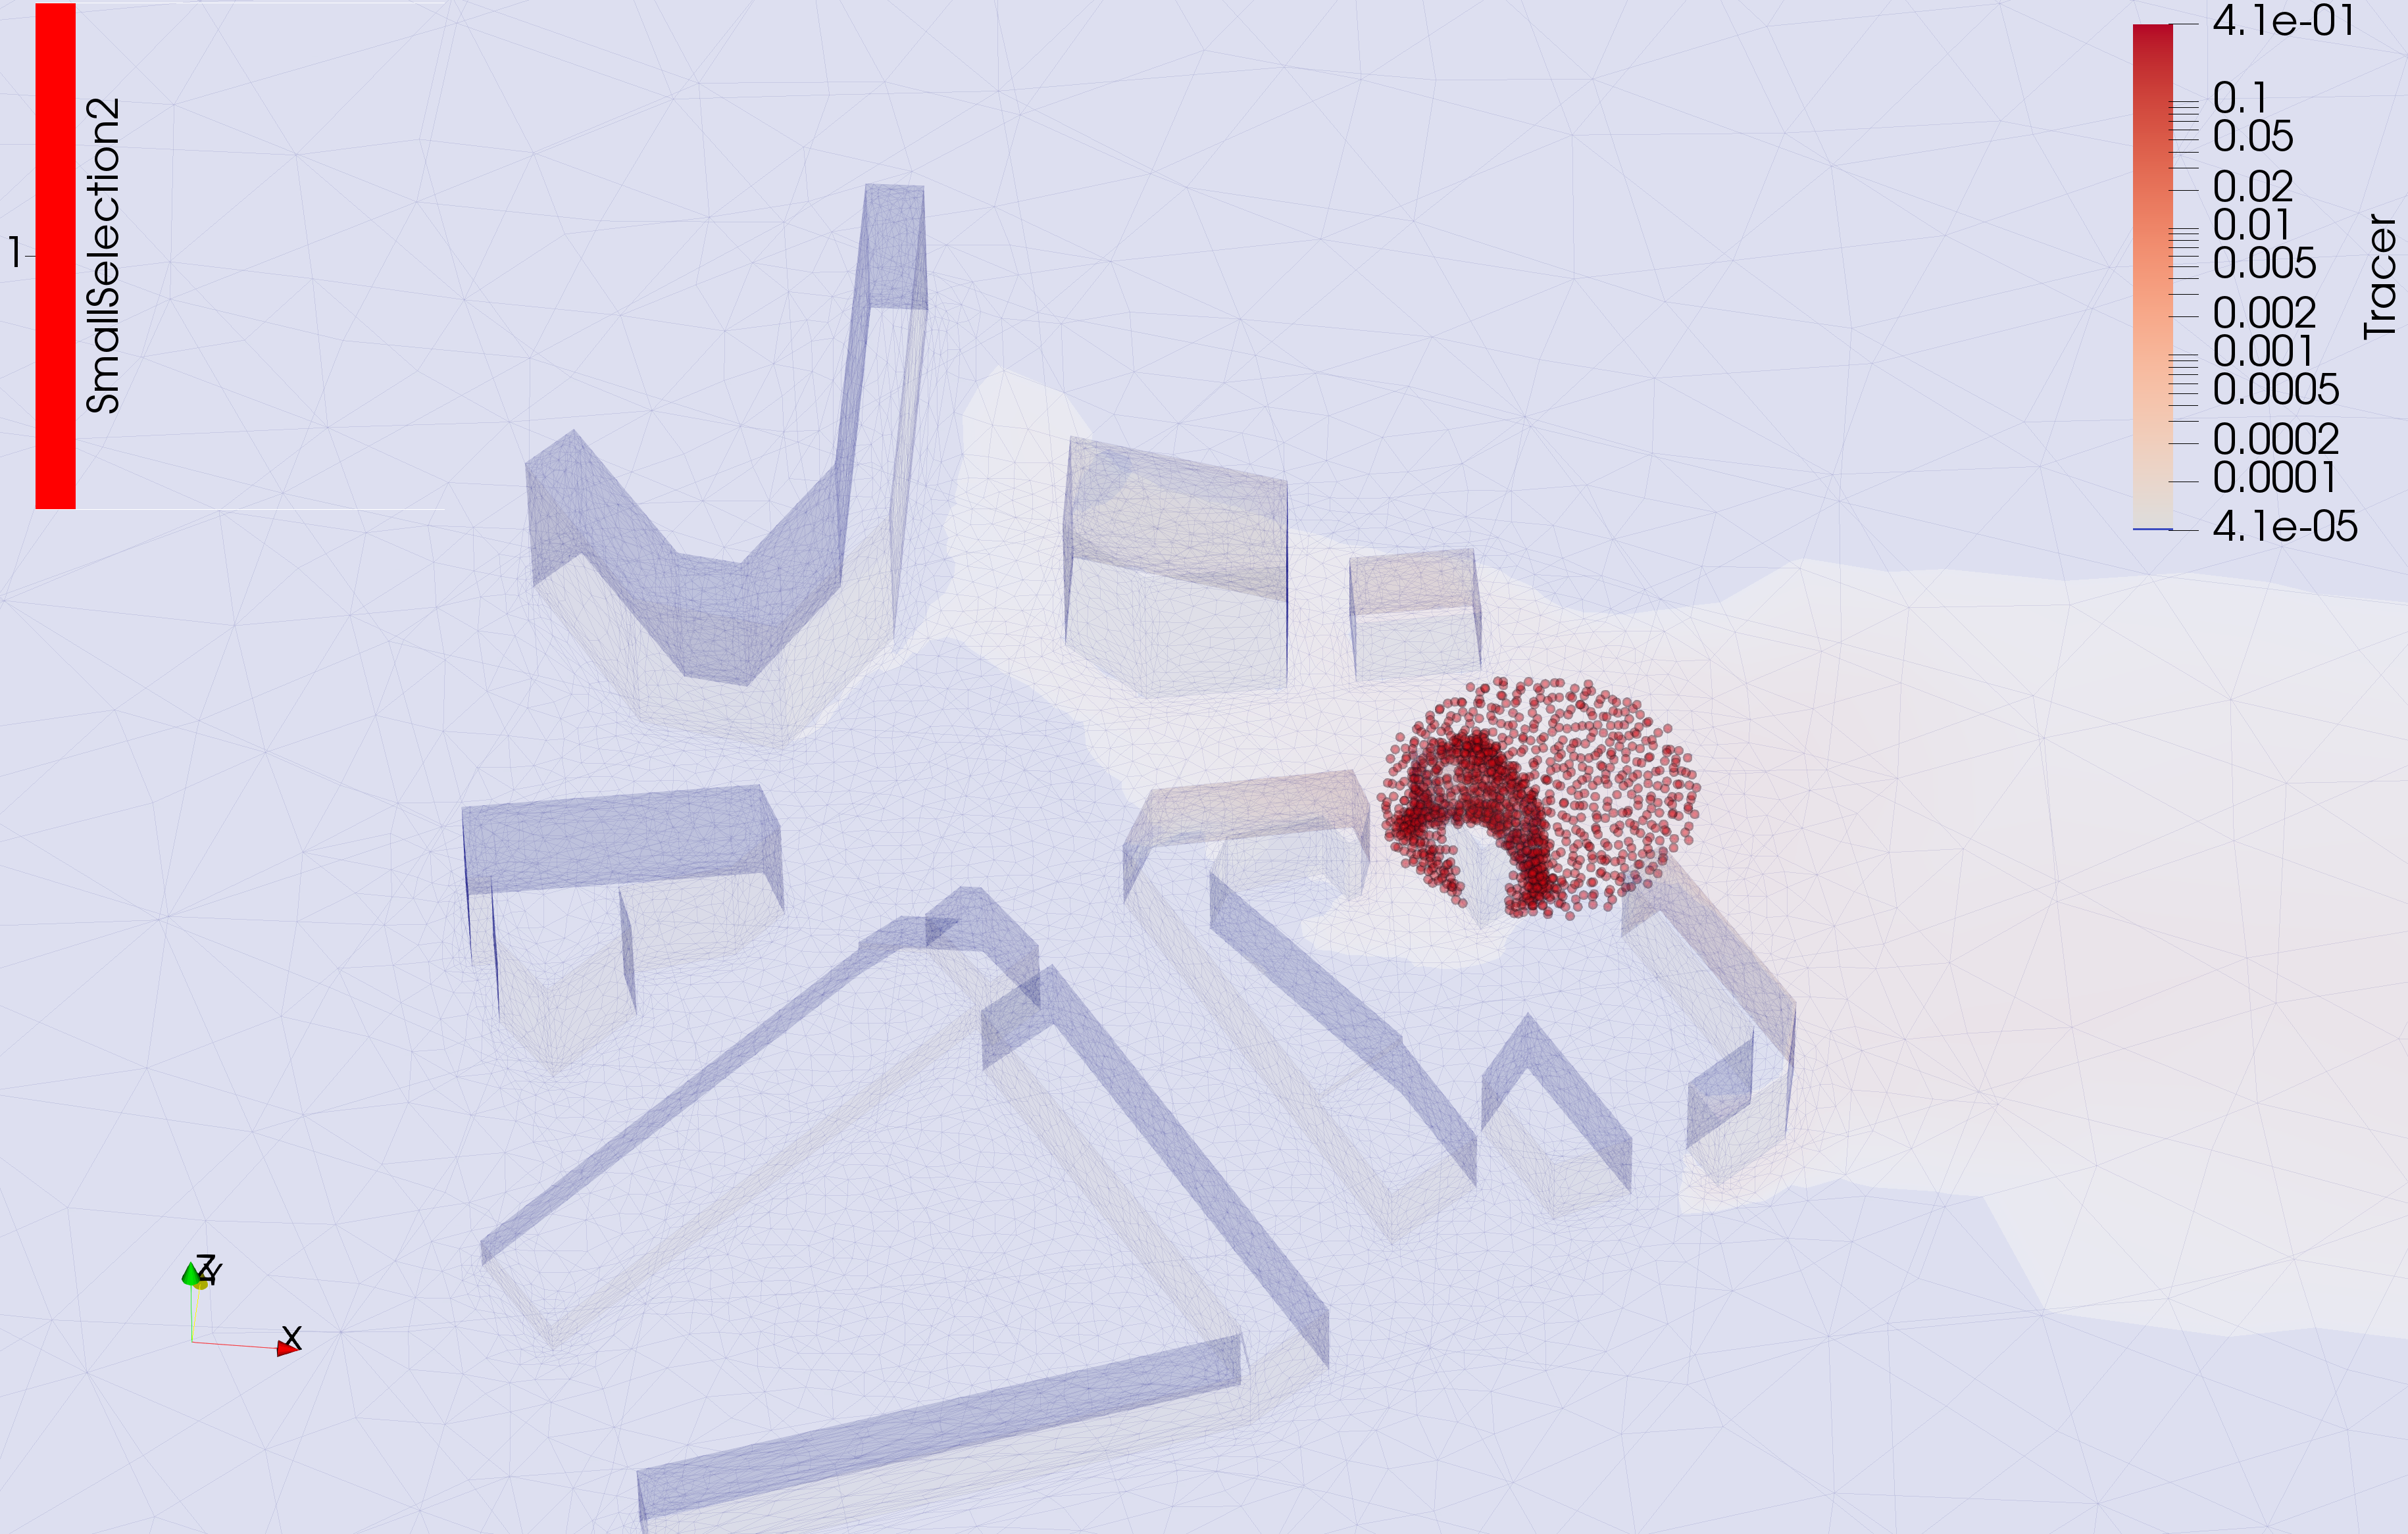
\includegraphics[width=0.8\linewidth]{figures/CompAlg/3rd/non_centered_60.35.0/candidates_screenshot}
	\caption{Small Subset Candidates}
\end{figure}

We compute the OAS covariance for this dataset and we will use in in the rest of the experience. The eigenvalues decomposition is shown for both the empirical covariance and the OAS estimate in the figure \ref{fig:small_cov_eig}. \\

\begin{figure}[h!]
\centering
	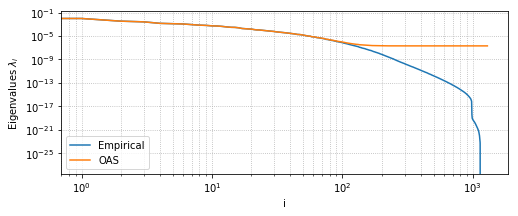
\includegraphics[width=0.7\linewidth]{figures/CompAlg/covarianceEmpOAS}
	\caption{Spectrum of Empirical and OAS covariances for small dataset}
	\label{fig:small_cov_eig}
\end{figure}

Next, we are going to optimise in this space $k=10$ points with the different algorithms and compare them based on their computation time and their similarity. 

\subsection{Naive and Lazy Optimisation}

First we optimise using the two first algorithms, the naive and the lazy versions of the near optimal sensor positioning algorithms. We observe immediately that output sets given by the two methods are the same. The main difference is as expected the computation time which is much larger in the first algorithm. The Naive Optimisation gives a result after $1043.27$s and the Lazy Optimisation gives results after $153.51 $s. \\

The location of those points is shown in figure \ref{fig:opt_small} and table \ref{tab:opt_small}.

\begin{figure}[h!]
\centering
	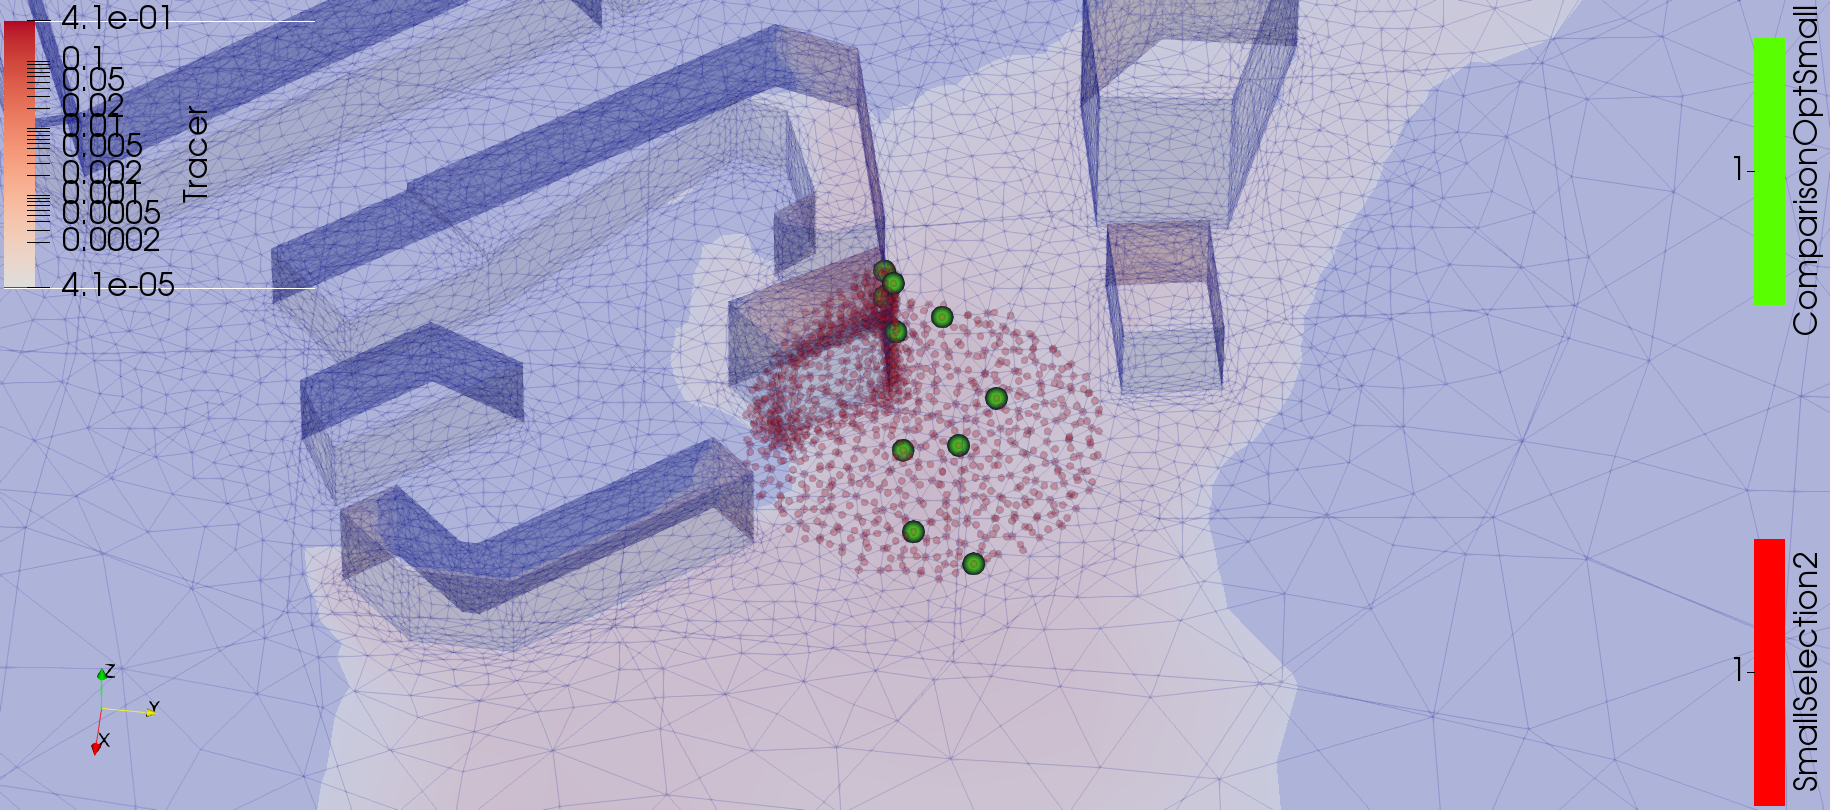
\includegraphics[width=0.8\linewidth]{figures/CompAlg/3rd/non_centered_60.35.0/optimal_screenshot}
	\caption{Optimal Points Location : Illustation}
	\label{fig:opt_small}
\end{figure}

\begin{table}[h]
\centering
\footnotesize
\begin{tabular}{|l|rrrrrrrrrr|}
\hline
idx &  52731 &  47876 &  3078  &  19782 &  26045 &  30511 &  26754 &  81507 &  11608 &  3903  \\
\hline
X &  61.31 &  43.55 &  77.31 &  38.75 &  48.23 &  50.48 &  52.36 &  43.10 &  82.40 &  62.01 \\
Y &  40.06 &  27.62 &  35.55 &  35.26 &  29.38 &  30.04 &  44.37 &  27.52 &  44.48 &  32.39 \\
Z &   1.52 &  16.40 &   1.45 &   1.80 &  19.53 &  11.79 &   1.62 &  10.23 &   1.96 &   0.20 \\
\hline
\end{tabular}
\caption{Optimal Points Locations : Data}
\label{tab:opt_small}
\end{table}

\subsection{Local Kernels Optimisation}

The 3rd Algorithm that we are going to use is the one that is scalable to larger datasets. This scalability is dependent on the parameter $\epsilon$, the thresholding parameter of the covariance. As the consequence the number of selected covariates $d$ is fluctuating and influences greatly the speed of the algorithm. This is why the threshold $\epsilon$ has to be chosen carefully. We are going to show that the speed, the accuracy and the parameter d varies according to $\epsilon$, before choosing a value that will be used for the full scale optimisation. \\


\begin{table}[h!]
\centering
\scriptsize
\begin{tabular}{|l|c|c|c|c|c|c|c|c|c|c|}
  \hline
  Threshold $\epsilon$ & $10^{-10} $ &  $10^{-9}$ & $10^{-8}$ & $10^{-7}$ & $10^{-6}$ & $10^{-5}$ & $10^{-4}$ & $10^{-3}$ & $10^{-2}$ & $10^{-1}$ \\
    \hline
  Distance [m]       &    0.00 &    0.00 &    0.00 &    0.00 &   12.48 &  27.83 & 46.93 & 110.58 & 110.58 & 110.58 \\
Time [s]       & 1660.85 & 1617.92 & 1500.63 & 1151.68 &  520.36 &  60.88 &  2.44 &   1.74 &   3.25 &   2.13 \\
Average d & 1289.40 & 1288.20 & 1284.80 & 1245.60 & 1029.60 & 510.50 & 15.20 &   0.00 &   0.00 &   0.00 \\
  \hline
\end{tabular}
\caption{Local Kernel Results}
\end{table}
\todo{Explain better d by referring to the equation}

We see that computation time is correlated with the average number of correlates d. For a threshold bellow $10^{-7}$, we see that the algorithm selects almost every point available and therefore we have computation times of the order of the naive algorithm. The optimised set of points is then also exactly the same as the naive and lazy algorithms. By increasing the threshold, we find that the computation time and number of covariates decreases at the expense of the accuracy represented by the increase in the distance between the found dataset and the optimal one.  \\

Therefore we need to \textbf{fix the threshold} at around $ \epsilon_{opt} = 10^{-6}$, so that the error is still small and the computation time substantially reduced. \\ 



\begin{figure}
\centering
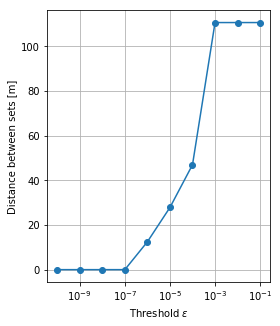
\includegraphics[height=0.33\linewidth]{figures/CompAlg/3rd/non_centered_60.35.0/comp_dist}
~
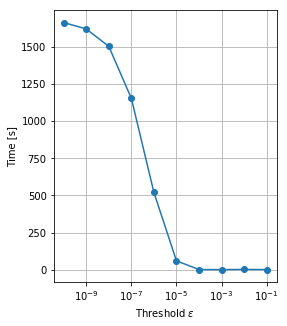
\includegraphics[height=0.33\linewidth]{figures/CompAlg/3rd/non_centered_60.35.0/comp_Time}
~
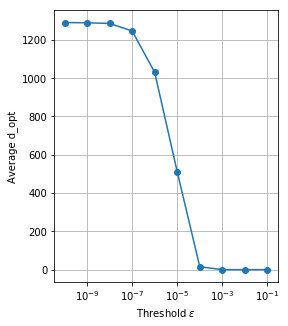
\includegraphics[height=0.33\linewidth]{figures/CompAlg/3rd/non_centered_60.35.0/comp_d_opt}
\caption{Local Kernels : Distance, Time and d, in function of $\epsilon$}
\end{figure}

By moving the center of the selection sphere, we observe that the optimal threshold is very different from one zone to the other. For example, if we place the subset in a zone where the tracer data is almost always null, we see that the threshold needs to be much smaller in order to get results. This is why the value we have chosen was optimised for an area where there is some data. 


\subsection{Approximated Gaussian Processes}

Alternatively, we use the approximation method developped earlier relying on the TSVD 

\subsection{Arbitrary Covariance}

Alternatively, we define the 

%\todo{Add section on the abritrary kernels results}




%%%%%%%%% OPTIMISATION %%%%%%%%

\section{Optimisation Results}

In this section we present the results of the optimisation done with 

\subsection{}

\subsection{Lazy Algorithm with TSVD}

\subsection{Local Kernel Algorithm}

\subsection{Local Kernel Algorithm}




%%%%%%%%% OPTIMISATION %%%%%%%%

\section{Validation with Data Assimilation}